\documentclass[10pt,xcolor=pdflatex]{beamer}
\usepackage{newcent}
\usepackage[utf8]{inputenc}
\usepackage[czech]{babel}
\usepackage{hyperref}
\usepackage{fancyvrb}
\usepackage{graphicx}
\usepackage{appendixnumberbeamer}
\graphicspath{ {./img/} }
\usetheme{FIT}

%%%%%%%%%%%%%%%%%%%%%%%%%%%%%%%%%%%%%%%%%%%%%%%%%%%%%%%%%%%%%%%%%%
\title[Aktualizace portálu evropských projektů a jeho rozšíření o identifikaci výsledků, souvisejících s tématy nově vypisovaných výzev]{Aktualizace portálu evropských projektů a jeho rozšíření o identifikaci výsledků, souvisejících s tématy nově vypisovaných výzev}

\author[Jiří Furda]{Jiří Furda\\*doc. RNDr. Pavel Smrž, Ph.D.}

\institute[FIT VUT]{Fakulta informačních technologií Vysokého učení technického v Brně\\
Bo\v{z}et\v{e}chova 1/2. 612 66 Brno - Kr\'alovo Pole\\
xfurda00@stud.fit.vutbr.cz}

\date{12. června 2019}
%\date{\today}
%\date{} % bez data

%%%%%%%%%%%%%%%%%%%%%%%%%%%%%%%%%%%%%%%%%%%%%%%%%%%%%%%%%%%%%%%%%%

\begin{document}

\frame[plain]{\titlepage}

\begin{frame}
    \frametitle{Motivace}
    \begin{itemize}
        \item Rozšíření možností portálu evropských projektů
            \begin{itemize}
                \item Např. přehled nejaktivnějších partnerů projektů v oblasti výzev obsahujících klíčové slovo \uv{space}
        	\end{itemize}
	\end{itemize}
	\begin{center}
	    
\includegraphics[height=5cm]{img/participants_summary.png}
        \vspace{0.3cm}
        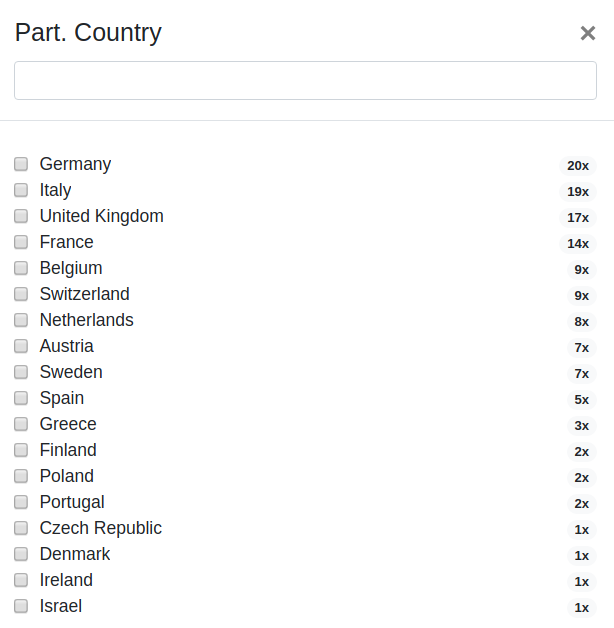
\includegraphics[height=5cm]{img/countries_summary.png}
    \end{center}
\end{frame}

\begin{frame}
    \frametitle{Cíle práce}
    \begin{itemize}
        \item Nastudování problematiky
            \begin{itemize}
                \item Indexace webových dat
                \item Dostupné řešení portálu
        	\end{itemize}
        \item Technologická aktualizace původního portálu
            \begin{itemize}
                \item Přechod z \emph{ElasticUtils} na \emph{Elasticsearch DSL}
                \item Nová implementace portálu 
                \item Nové uživatelské rozhraní
        	\end{itemize}
    	\item Rozšíření poskytovaného obsahu
    	    \begin{itemize}
                \item Začlenění témat výzev pro podávání návrhů nových projektů
        	\end{itemize}
	\end{itemize}
\end{frame}

\begin{frame}
    \frametitle{Schéma systému}
    \begin{center}
        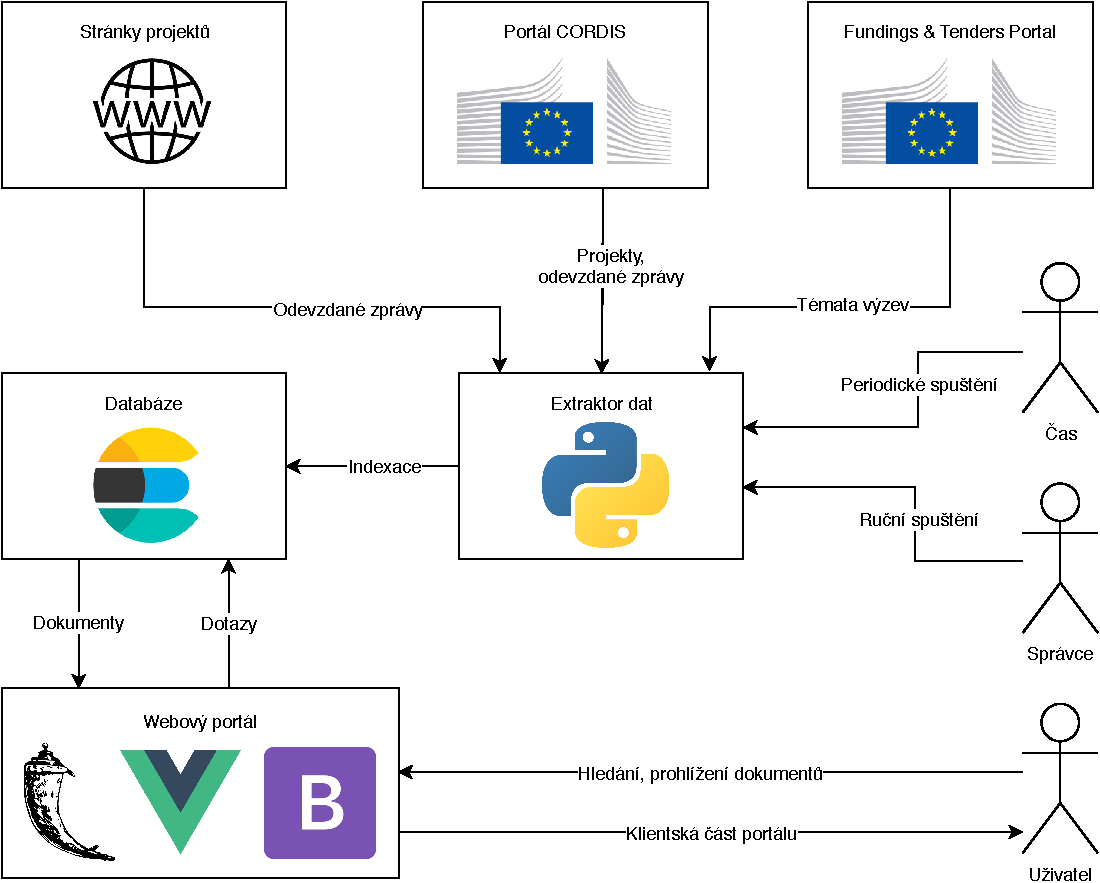
\includegraphics[scale=0.5]{img/my-scheme.pdf}
    \end{center}
\end{frame}

\begin{frame}
    \frametitle{Výsledný portál}
    \begin{center}
        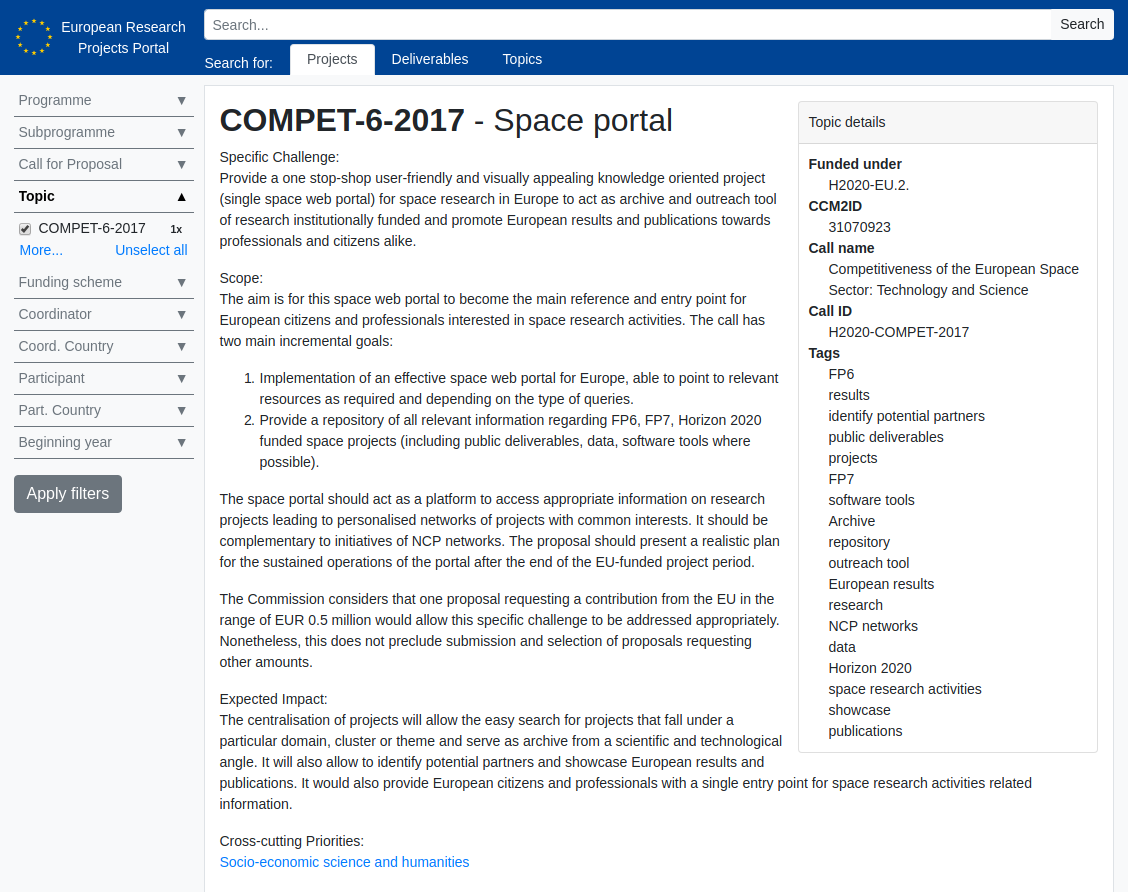
\includegraphics[scale=0.25]{img/my-topic.png}
    \end{center}
\end{frame}

\begin{frame}
    \frametitle{Vyhodnocení}
     \begin{itemize}
        \item Ukázka vyhodnocení rozhraní ze strany uživatele
    \end{itemize}
    \begin{center}
        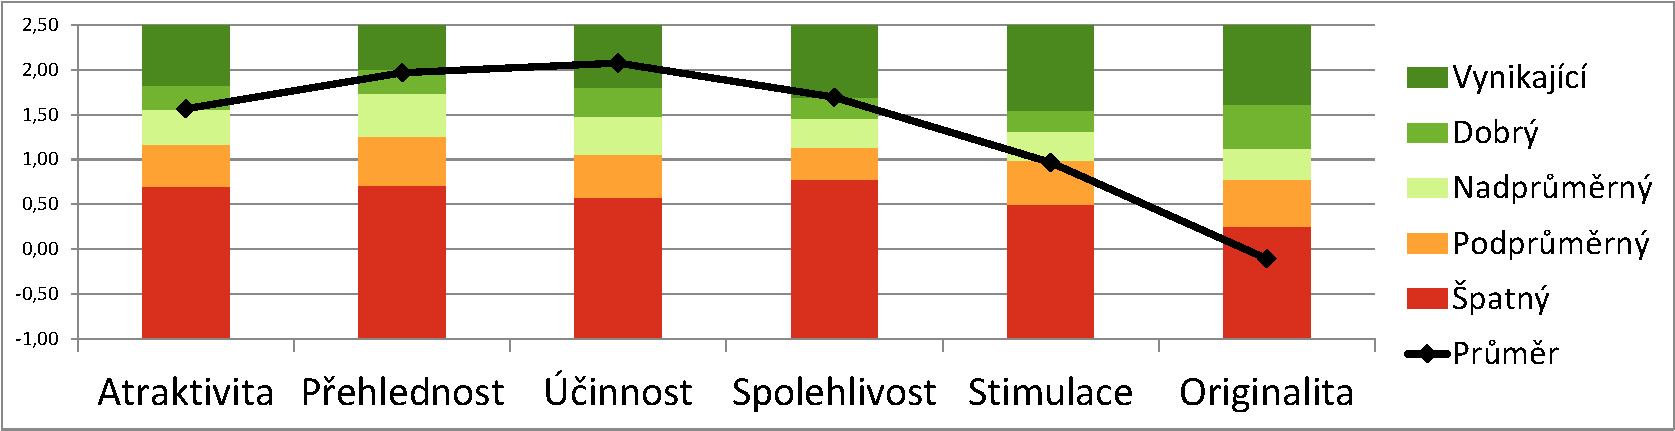
\includegraphics[width=\textwidth]{img/ueq-benchmark.pdf}
    \end{center}
    \begin{table}[H]
        \centering
        \begin{tabular}{ |l|c|l|l| } 
        \hline
        Aspekt       & Průměr & Výsledek    \\
        \hline
        Atraktivita  & 1.57   & Dobrý       \\
        Přehlednost  & 1.97   & Vynikající  \\
        Účinnost     & 2.08   & Vynikající  \\
        Spolehlivost & 1.70   & Vynikající  \\
        Stimulace    & 0.97   & Podprůměrný \\
        Originalita  & -0.11  & Špatný      \\  
        \hline
        \end{tabular}
    \end{table}
\end{frame}

\begin{frame}
    \frametitle{Shrnutí}
    \begin{itemize}
        \item Zakomponování výzev k podávání projektů
        \begin{itemize}
            \item Fasetového i plnotextového vyhledávání
            \item Pokročilé vyhledávání pomocí \emph{query\_string}
        \end{itemize}
        
        \item Nové grafické rozhraní
        \begin{itemize}
            \item Přehlednější fasetová navigace
        \end{itemize}
        
        \item Portál pracuje s novějšími technologiemi
        \begin{itemize}
            \item Elasticsearch, Elasticsearch DSL
            \item Vue.js, BootstrapVue
        \end{itemize}

    \end{itemize}
\end{frame}

\appendix

\begin{frame}[plain,noframenumbering]
    \frametitle{Otázka oponenta č. 1}
    \emph{Aké sú problémy pri sťahovaní a indexácií dát z portálu o európskych projektoch a ako by ich šlo riešiť?}
    \begin{itemize}
        \item Chybějící hodnoty u některých položek
        \begin{itemize}
            \item Robustní programování předcházející tyto situace
        \end{itemize}
        \item Výzvy rozdělené do více částí
        \begin{itemize}
            \item Každá část je prezentována jako samostatná výzva
            \item Všechny části sdílí jednu stránku detailu
        \end{itemize}
    \end{itemize}
\end{frame}

\begin{frame}[plain,noframenumbering]
    \frametitle{Otázka oponenta č. 2}
    \emph{Rozmýšlal študent nad tým ako efektívne s portálom bude pracovať užívateľ, resp. skúsil porovnať sposôb práce v jeho systéme a iných existujúcich systémoch?}
    \begin{itemize}
        \item The Funding \& Tenders Portal má velmi omezené možnosti vyhledávání.
        \item Chybí zejména:
        \begin{itemize}
            \item Pokročilý dotazovací jazyk
            \item Plnotextové vyhledávání
            \item Náhledy výsledků
        \end{itemize}
    \end{itemize}
\end{frame}

\begin{frame}[plain,noframenumbering]
    \frametitle{Otázka oponenta č. 2}

    The Funding \& Tenders Portal
    \begin{center}
        
\includegraphics[width=\textwidth]{img/funding_search_result.png}
    \end{center}

    \vspace{0.5cm}
    
    Mé řešení
    \begin{center}
        
\includegraphics[width=\textwidth]{img/my_search_result.png}
    \end{center}
\end{frame}

\end{document}

